\documentclass[border=10pt]{standalone}
\usepackage{tikz}
\usetikzlibrary{er, positioning, fit, calc, shapes.geometric}

\begin{document}

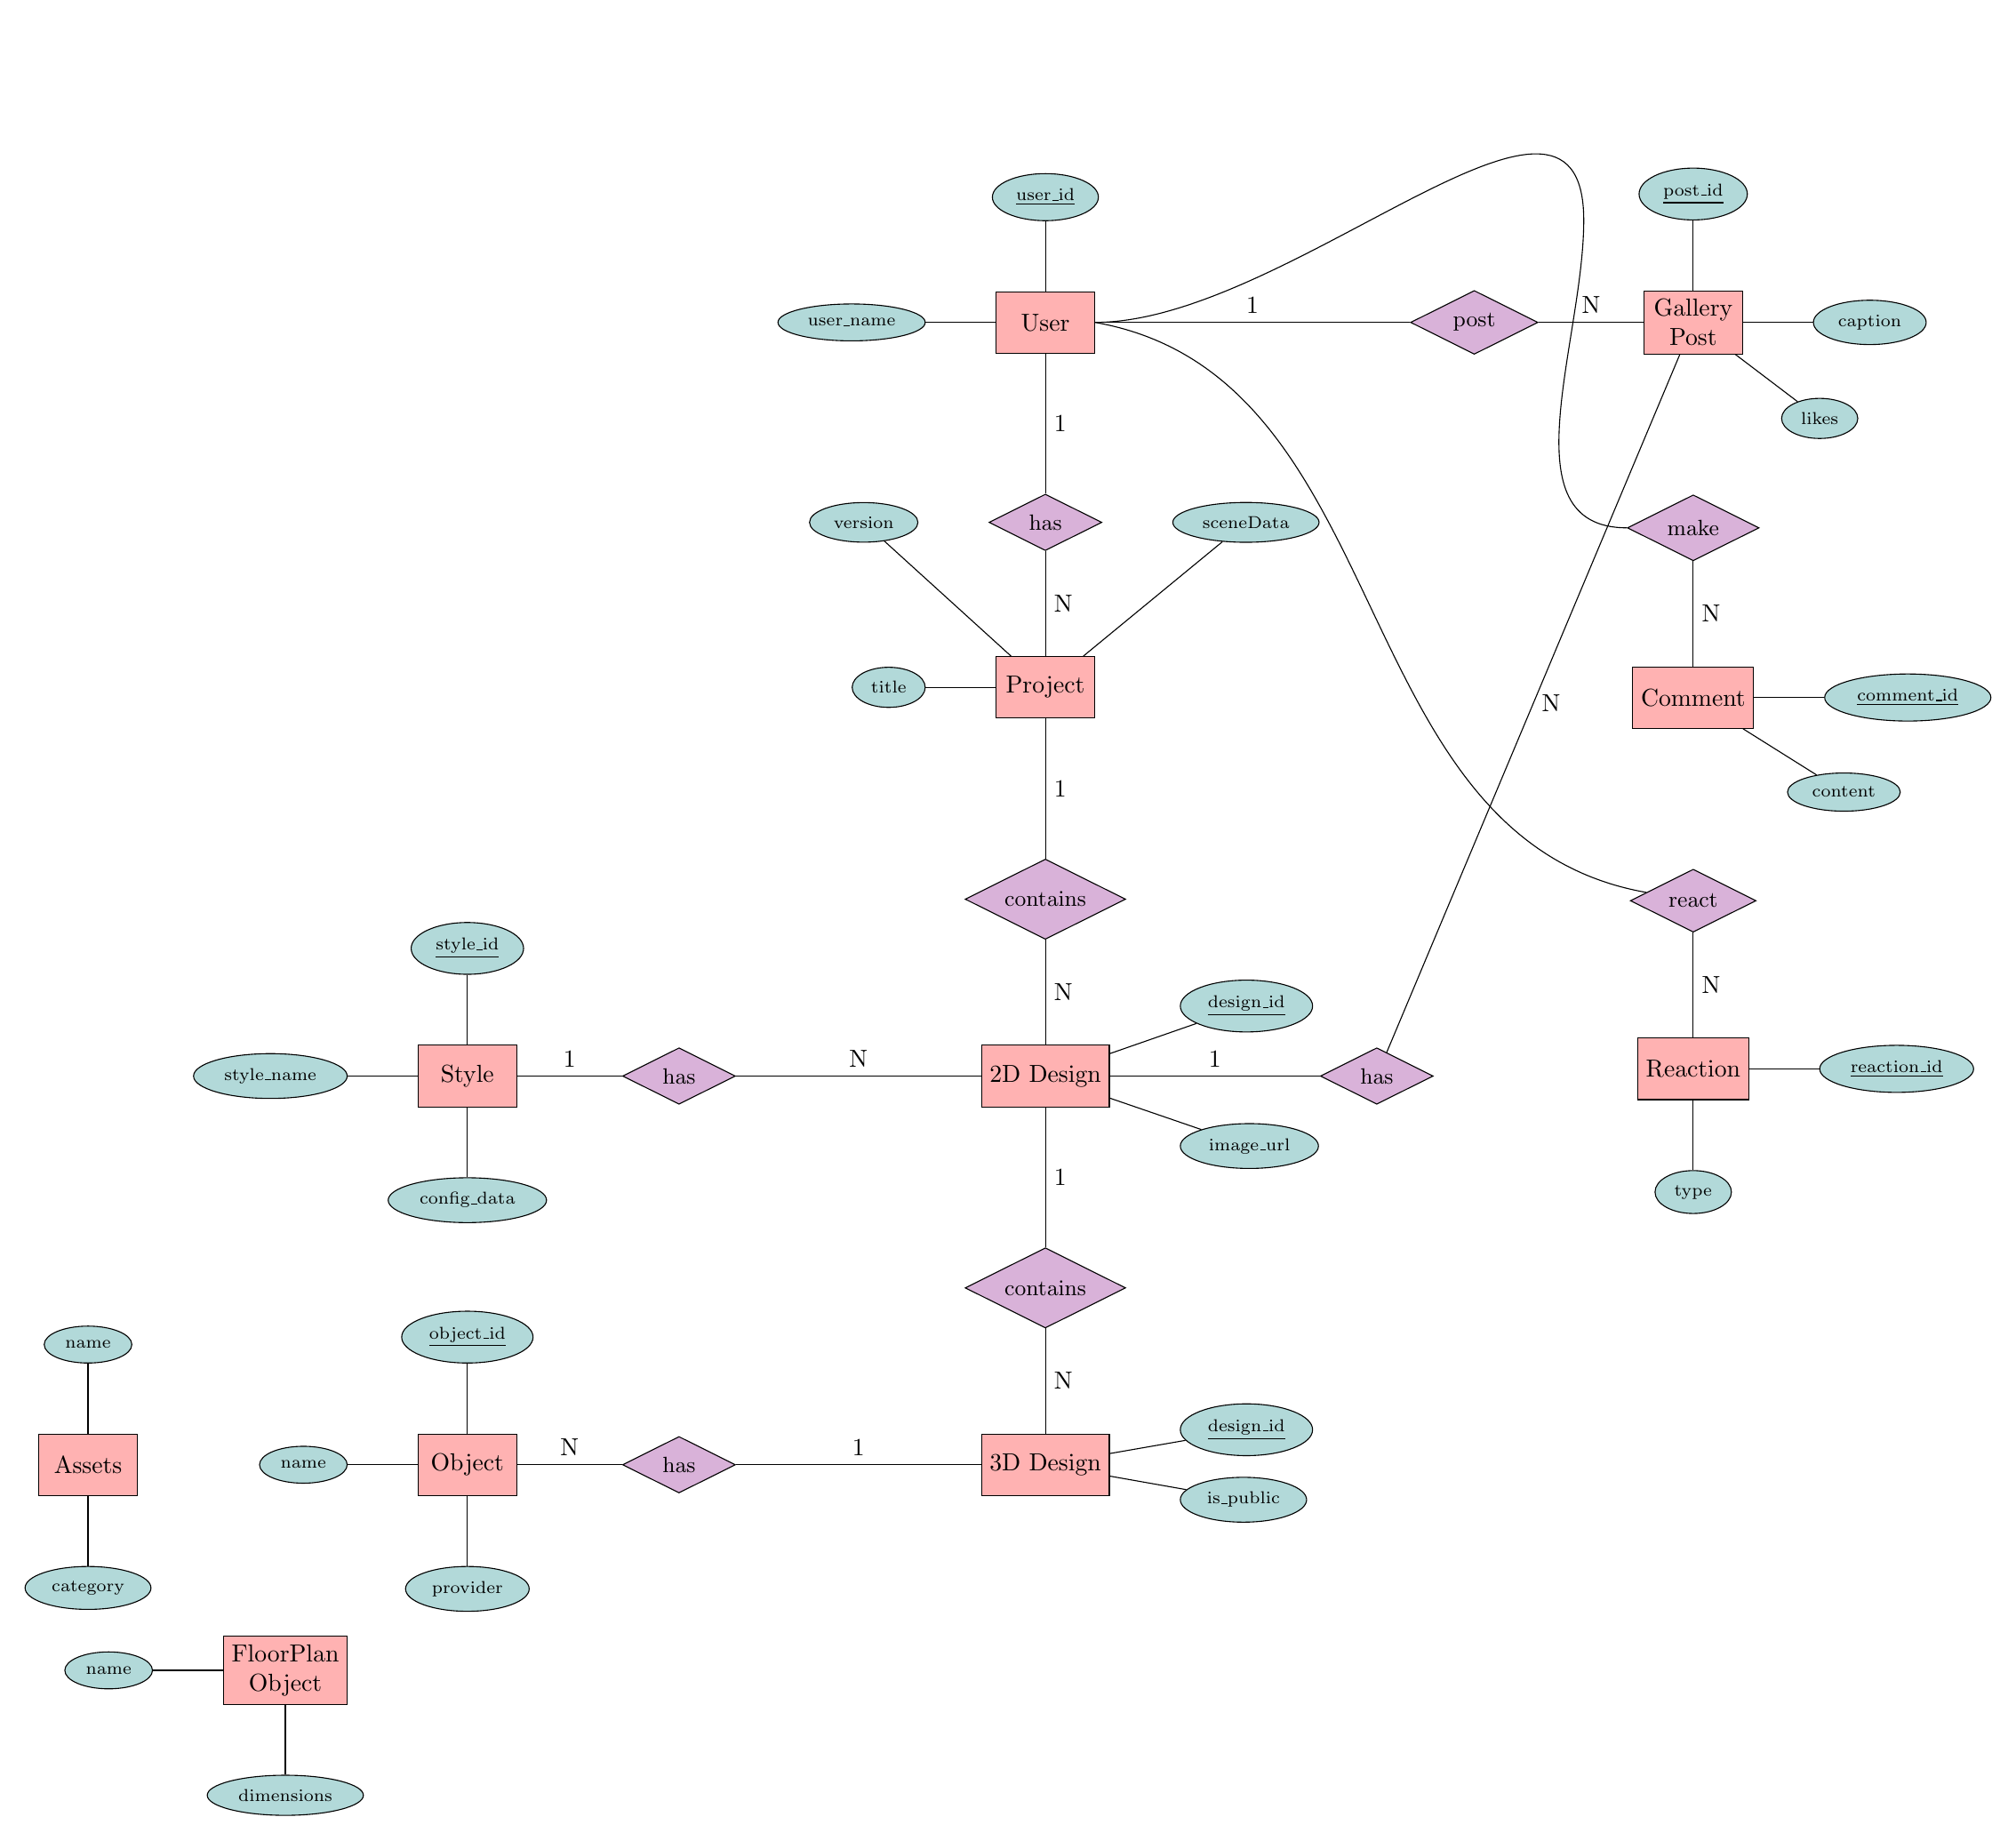
\begin{tikzpicture}[
    node distance=2cm,
    entity/.style={
        draw, 
        rectangle, 
        fill=red!30, 
        minimum height=2.5em, 
        minimum width=4em, 
        align=center
    },
    weak entity/.style={
        entity,
        double,
        double distance=2pt
    },
    attribute/.style={
        draw, 
        ellipse, 
        fill=teal!30, 
        minimum height=1.5em, 
        align=center,
        font=\scriptsize
    },
    relationship/.style={
        draw, 
        diamond, 
        fill=violet!30, 
        aspect=2, 
        minimum height=1.5em, 
        align=center,
        font=\small
    },
    weak relationship/.style={
        relationship,
        double,
        double distance=2pt
    },
    every edge/.style={
        draw, 
        thick
    }
]

    % ---------------------------------------------------------
    % 1. ANCHOR: USER (Top Center)
    % ---------------------------------------------------------
    \node[entity] (user) {User};
    \node[attribute] (uid) [above=1cm of user] {\underline{user\_id}};
    \node[attribute] (uname) [left=1cm of user] {user\_name};
    \draw (user) -- (uid);
    \draw (user) -- (uname);

    % ---------------------------------------------------------
    % 2. SOCIAL WING (Right Side)
    % ---------------------------------------------------------
    % Pushed further right (4.5cm) to prevent line crossing overlap
    
    % Gallery Post
    \node[relationship] (post_rel) [right=4.5cm of user] {post};
    \node[entity] (gallery) [right=1.5cm of post_rel] {Gallery\\Post};
    
    % Gallery Attributes
    \node[attribute] (gid) [above=1cm of gallery] {\underline{post\_id}};
    \node[attribute] (gcap) [right=1cm of gallery] {caption};
    \node[attribute] (glike) [below right=1cm of gallery] {likes};
    
    \draw (user) -- node[above]{1} (post_rel);
    \draw (post_rel) -- node[above]{N} (gallery);
    \draw (gallery) -- (gid);
    \draw (gallery) -- (gcap);
    \draw (gallery) -- (glike);

    % Comment (Below Gallery)
    \node[relationship] (make_comm) [below=2cm of gallery] {make};
    \node[entity] (comment) [below=1.5cm of make_comm] {Comment};
    \node[attribute] (cid) [right=1cm of comment] {\underline{comment\_id}};
    \node[attribute] (ccont) [below right=1cm of comment] {content};
    
    % Line from User to Comment
    \draw (user.east) to[out=0,in=90] ($(post_rel.north)!0.5!(gallery.north) + (0, 1)$) to[out=-90, in=180] (make_comm);
    \draw (make_comm) -- node[right]{N} (comment);
    \draw (comment) -- (cid);
    \draw (comment) -- (ccont);

    % Reaction (Below Comment)
    \node[relationship] (do_react) [below=2cm of comment] {react};
    \node[entity] (reaction) [below=1.5cm of do_react] {Reaction};
    \node[attribute] (rid) [right=1cm of reaction] {\underline{reaction\_id}};
    \node[attribute] (rtype) [below=1cm of reaction] {type};
    
    % Line from User to Reaction
    % Routing lines carefully to avoid cutting through other shapes
    \draw (user.east) to[out=-10,in=170] (do_react);
    \draw (do_react) -- node[right]{N} (reaction);
    \draw (reaction) -- (rid);
    \draw (reaction) -- (rtype);

    % ---------------------------------------------------------
    % 3. DESIGN SPINE (Center Down)
    % ---------------------------------------------------------

    % Project
    \node[relationship] (has_proj) [below=2cm of user] {has};
    \node[entity] (project) [below=1.5cm of has_proj] {Project};
    
    % Project Attributes
    \node[attribute] (ptitle) [left=1cm of project] {title};
    \node[attribute] (pver) [left=1cm of has_proj] {version};
    \node[attribute] (pscene) [right=1cm of has_proj] {sceneData};
    
    \draw (user) -- node[right]{1} (has_proj);
    \draw (has_proj) -- node[right]{N} (project);
    \draw (project) -- (ptitle);
    \draw (project) -- (pver);
    \draw (project) -- (pscene);

    % 2D Design
    \node[relationship] (has_2d) [below=2cm of project] {contains};
    \node[entity] (design2d) [below=1.5cm of has_2d] {2D Design};
    
    % FIXED: Moved design_id to RIGHT to avoid collision with Style
    \node[attribute] (d2id) [right=1cm of design2d, yshift=1cm] {\underline{design\_id}};
    \node[attribute] (d2img) [right=1cm of design2d, yshift=-1cm] {image\_url};
    
    \draw (project) -- node[right]{1} (has_2d);
    \draw (has_2d) -- node[right]{N} (design2d);
    \draw (design2d) -- (d2id);
    \draw (design2d) -- (d2img);

    % Link 2D Design to Gallery
    \node[relationship] (shown_in) [right=3cm of design2d] {has};
    \draw (design2d) -- node[above]{1} (shown_in);
    \draw (shown_in) -- node[right]{N} (gallery);

    % 3D Design
    \node[relationship] (has_3d) [below=2cm of design2d] {contains};
    \node[entity] (design3d) [below=1.5cm of has_3d] {3D Design};
    
    % FIXED: Moved design_id to RIGHT to avoid collision with Object
    \node[attribute] (d3id) [right=1cm of design3d, yshift=0.5cm] {\underline{design\_id}};
    \node[attribute] (d3pub) [right=1cm of design3d, yshift=-0.5cm] {is\_public};
    
    \draw (design2d) -- node[right]{1} (has_3d);
    \draw (has_3d) -- node[right]{N} (design3d);
    \draw (design3d) -- (d3id);
    \draw (design3d) -- (d3pub);

    % ---------------------------------------------------------
    % 4. ASSET WING (Left Side)
    % ---------------------------------------------------------

    % Style (Connected to 2D Design)
    \node[relationship] (uses_style) [left=3.5cm of design2d] {has};
    \node[entity] (style) [left=1.5cm of uses_style] {Style};
    
    \node[attribute] (sid) [above=1cm of style] {\underline{style\_id}};
    \node[attribute] (sname) [left=1cm of style] {style\_name};
    \node[attribute] (sconf) [below=1cm of style] {config\_data};
    
    \draw (design2d) -- node[above]{N} (uses_style);
    \draw (uses_style) -- node[above]{1} (style);
    \draw (style) -- (sid);
    \draw (style) -- (sname);
    \draw (style) -- (sconf);

    % Object (Connected to 3D Design)
    \node[relationship] (uses_obj) [left=3.5cm of design3d] {has};
    \node[entity] (object) [left=1.5cm of uses_obj] {Object};
    
    \node[attribute] (oid) [above=1cm of object] {\underline{object\_id}};
    \node[attribute] (oname) [left=1cm of object] {name};
    \node[attribute] (opro) [below=1cm of object] {provider};
    
    \draw (design3d) -- node[above]{1} (uses_obj);
    \draw (uses_obj) -- node[above]{N} (object);
    \draw (object) -- (oid);
    \draw (object) -- (oname);
    \draw (object) -- (opro);

    % FloorPlan Object (Floating/Related)
    \node[entity] (floor) [below left=2cm and 1cm of object] {FloorPlan\\Object};
    \node[attribute] (fname) [left=1cm of floor] {name};
    \node[attribute] (fdim) [below=1cm of floor] {dimensions};
    \draw (floor) -- (fname);
    \draw (floor) -- (fdim);

    % Assets (Floating/Related)
    \node[entity] (asset) [left=4cm of object] {Assets};
    \node[attribute] (aname) [above=1cm of asset] {name};
    \node[attribute] (acat) [below=1cm of asset] {category};
    \draw (asset) -- (aname);
    \draw (asset) -- (acat);

\end{tikzpicture}

\end{document}